\documentclass{beamer}
\usetheme{default}
\usepackage{graphicx}

\title{Mi camino para ser Debian Developer}
\author{Emmanuel Arias}
\date{18 de octubre de 2024}
\begin{document}
\begin{frame}[plain]
    \maketitle
\end{frame}
\begin{frame}
  \frametitle {Objetivo}
  \centering
    \Huge Seamos más miembros de Debian en Argentina!!!
\end{frame}
\begin{frame}
    \frametitle {Argentinos en Debian}
    \begin{itemize}
    	\item Agustin Henze
    	\item Marcela Tiznado
    	\item Lisandro Damián Nicanor Pérez Meyer *
    	\item Ulises Vitulli *
    	\item Jose Luis Rivas Contreras
    	\item Emmanuel Arias *
    \end{itemize}

    \vspace{1cm} \\
    \tiny Fuente: https://db.debian.org/
\end{frame}
\begin{frame}
  \frametitle{Argentinos en Debian}
  \centering
  \Huge 1 DD por cada 7.705.805
  \vspace{1cm} \\
  \tiny Fuente: https://www.argentina.gob.ar/pais/poblacion
\end{frame}
\begin{frame}
  \frametitle{Argentinos en Debian}
  \centering
  \Huge 1 DD por cada 915  (Si es que solo hay 5490 del área de sistema en
  Argentina)
  \vspace{1cm} \\
  \tiny Fuente: https://sueldos.openqube.io/encuesta-sueldos-2024.01/
\end{frame}

\begin{frame}
  \frametitle{¿Qué es Debian?}
	\begin{figure}
		\centering
		
\includegraphics[width=0.7\linewidth]{images/debian}
		\label{fig:debian}
	\end{figure}
\end{frame}
\begin{frame}
  \frametitle{Versiones de Debian}
	\begin{figure}
		\centering
		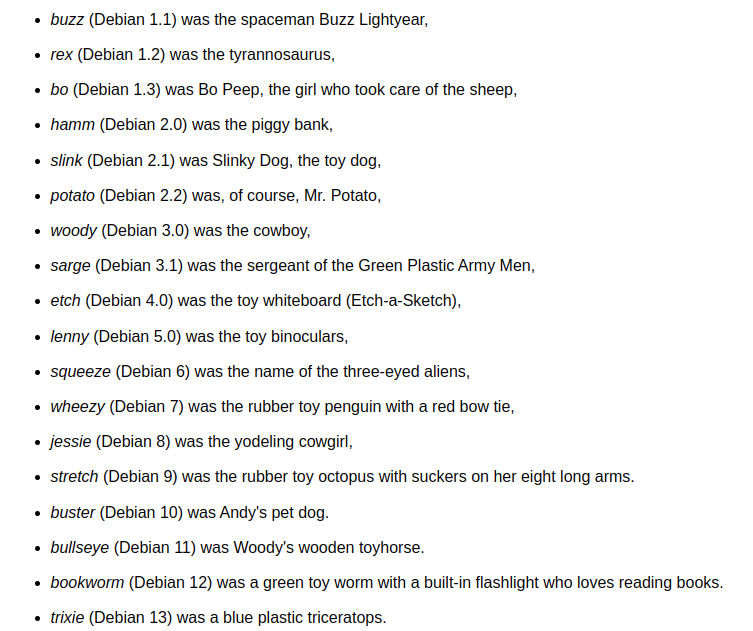
\includegraphics[width=0.7\linewidth]{images/versions.png}
		\label{fig:versiones de Debian}
	\end{figure}
\end{frame}
\begin{frame}
  \frametitle{Comunidad de Debian}
	\begin{figure}
		\centering
		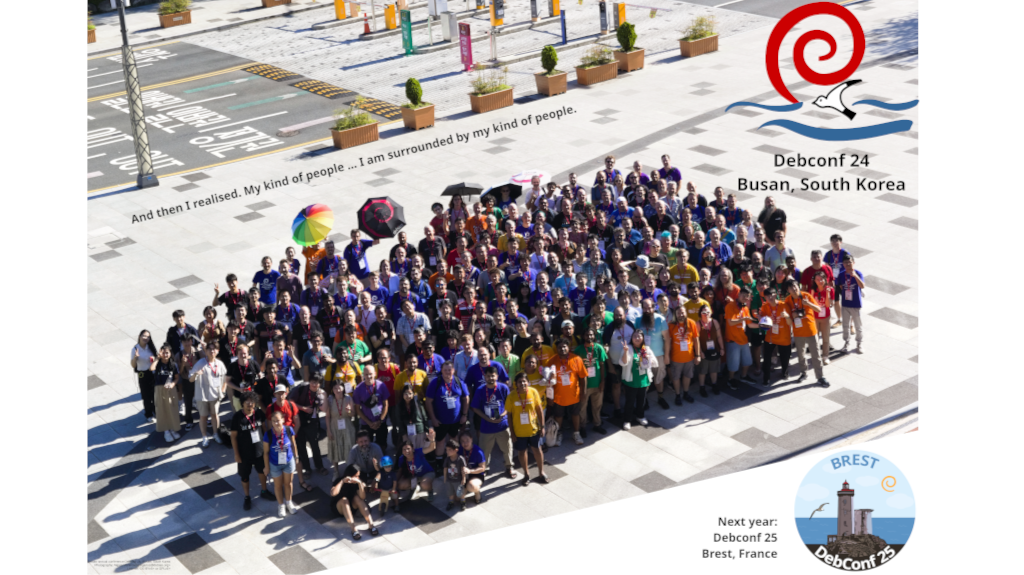
\includegraphics[width=0.7\linewidth]{images/debconf.png}
		\label{fig:comunidad de Debian}
	\end{figure}
\end{frame}

\begin{frame}%[allowframebreaks]
  \frametitle{¿Por qué contribuir a Debian?}
  \begin{itemize}
    \item A algunas personas, sencillamente, les gusta ayudar a los demás, y
      contribuir a un proyecto de software libre es una magnífica manera de
      hacerlo. \pause
    \item Muchos desarrolladores y desarrolladoras escriben programas para
      aprender más acerca de las computadoras, de las diferentes arquitecturas y
      de los lenguajes de programación. \pause
    \item Algunos desarrolladores contribuyen para decir ``''gracias'' por todo
      el excelente software libre que han recibido de otros. \pause
    \item Muchas personas en las instituciones académicas crean software libre
      para compartir el resultado de sus investigaciones. \pause
    \item Las empresas también ayudan a mantener software libre para influir en
      el desarrollo de aplicaciones o para implementar funcionalidades nuevas
      rápidamente. \pause
    \item Desde luego, ¡la mayoría de los desarrolladores de Debian participan
      porque les parece muy divertido!
  \end{itemize}
\end{frame}

\begin{frame}
 \centering
 \Huge Ok, ¿pero como empiezo?
\end{frame}
\begin{frame}
 \frametitle{Instalando un GNU/Linux}
    \begin{figure}
		\centering
		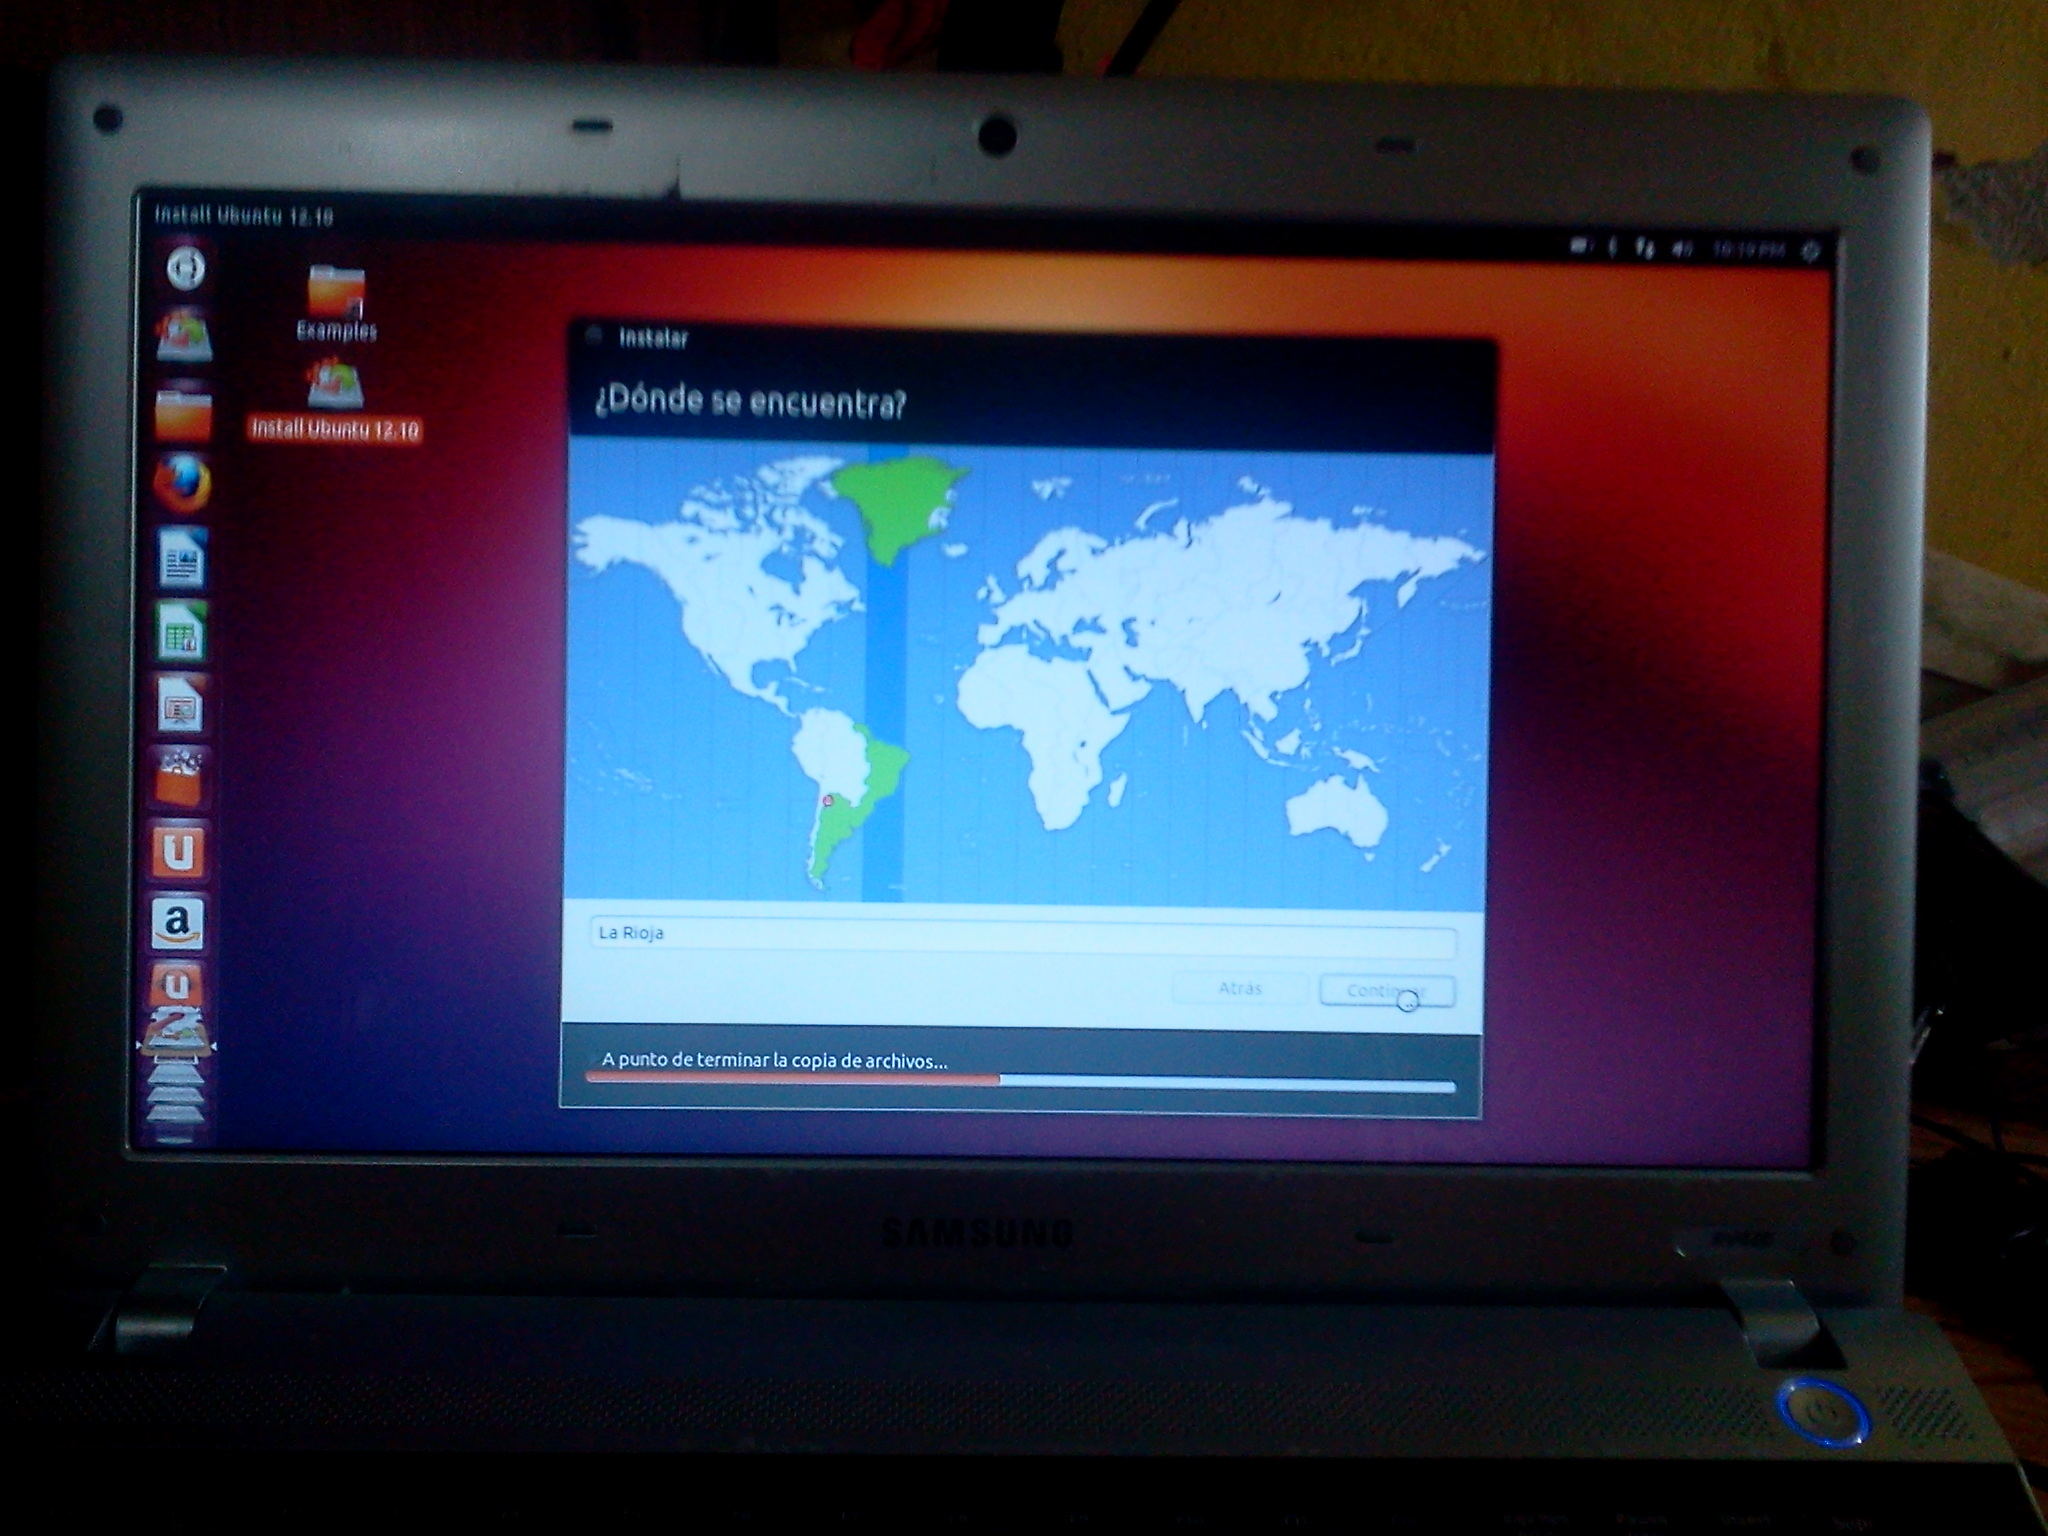
\includegraphics[width=0.7\linewidth]{images/ubuntu.jpg}
		\label{fig:Install Ubuntu}
	\end{figure}
\end{frame}

\begin{frame}
  \centering
  \Huge Usando Debian, hablando de Debian.
\end{frame}

\begin{frame}
  \centering
  \Huge Buscando personas que le guste Debian (o el software libre)
\end{frame}

\begin{frame}
\frametitle{Buscando paquetes que necesiten ayuda}
  \begin{itemize}
    \item O: Orphaned
    \item RFP: Request for package
    \item RFH: Request for help
    \item RFA: Request for adopt
  \end{itemize}
\end{frame}
\begin{frame}
 \frametitle{Orphaned}
    \begin{figure}
		\centering
		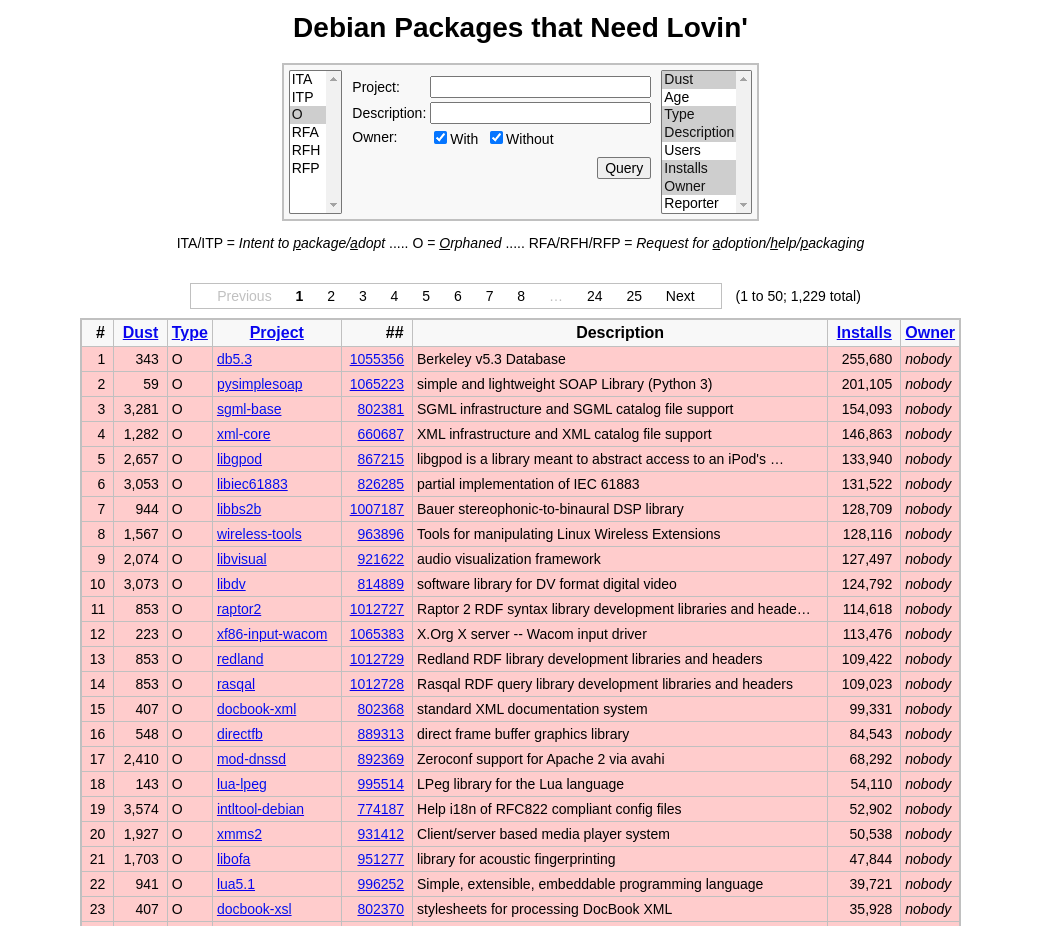
\includegraphics[width=0.7\linewidth]{images/orphaned}
		\label{fig:Orphaned}
	\end{figure}
\end{frame}

\begin{frame}
 \frametitle{RFA}
    \begin{figure}
		\centering
		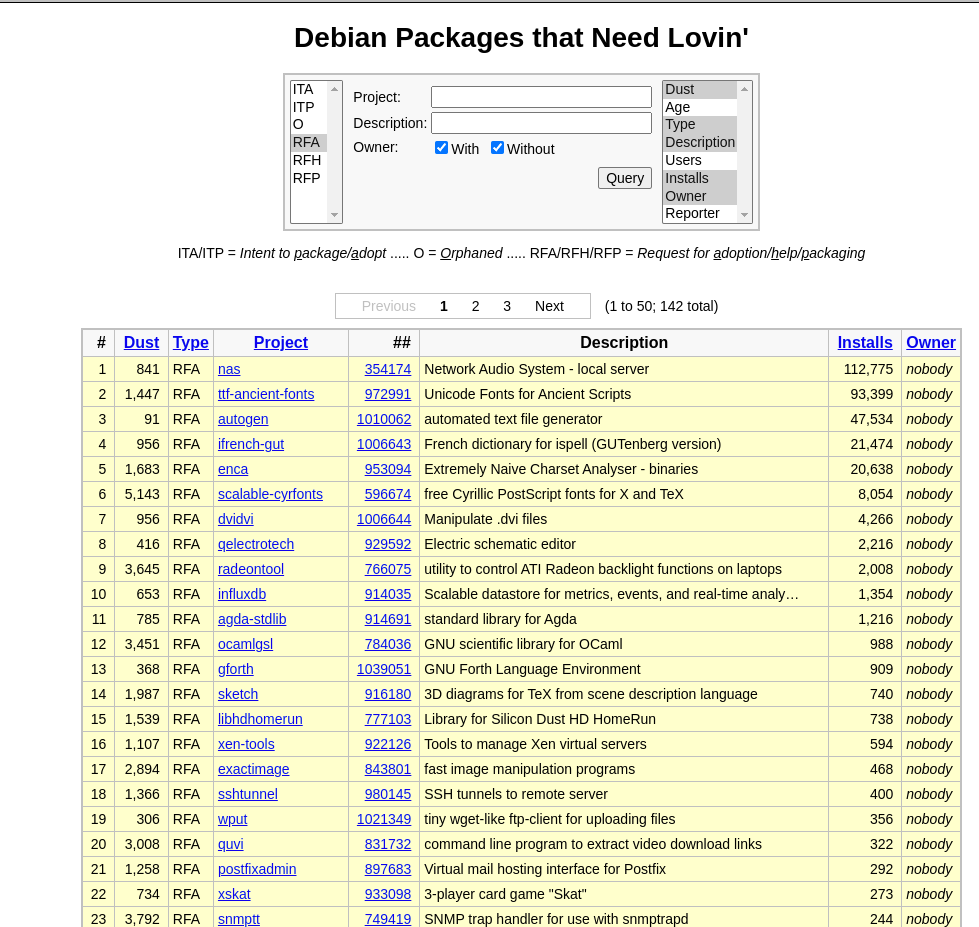
\includegraphics[width=0.7\linewidth]{images/rfa}
		\label{fig:rfa}
	\end{figure}
\end{frame}

\begin{frame}
 \frametitle{RFP}
    \begin{figure}
		\centering
		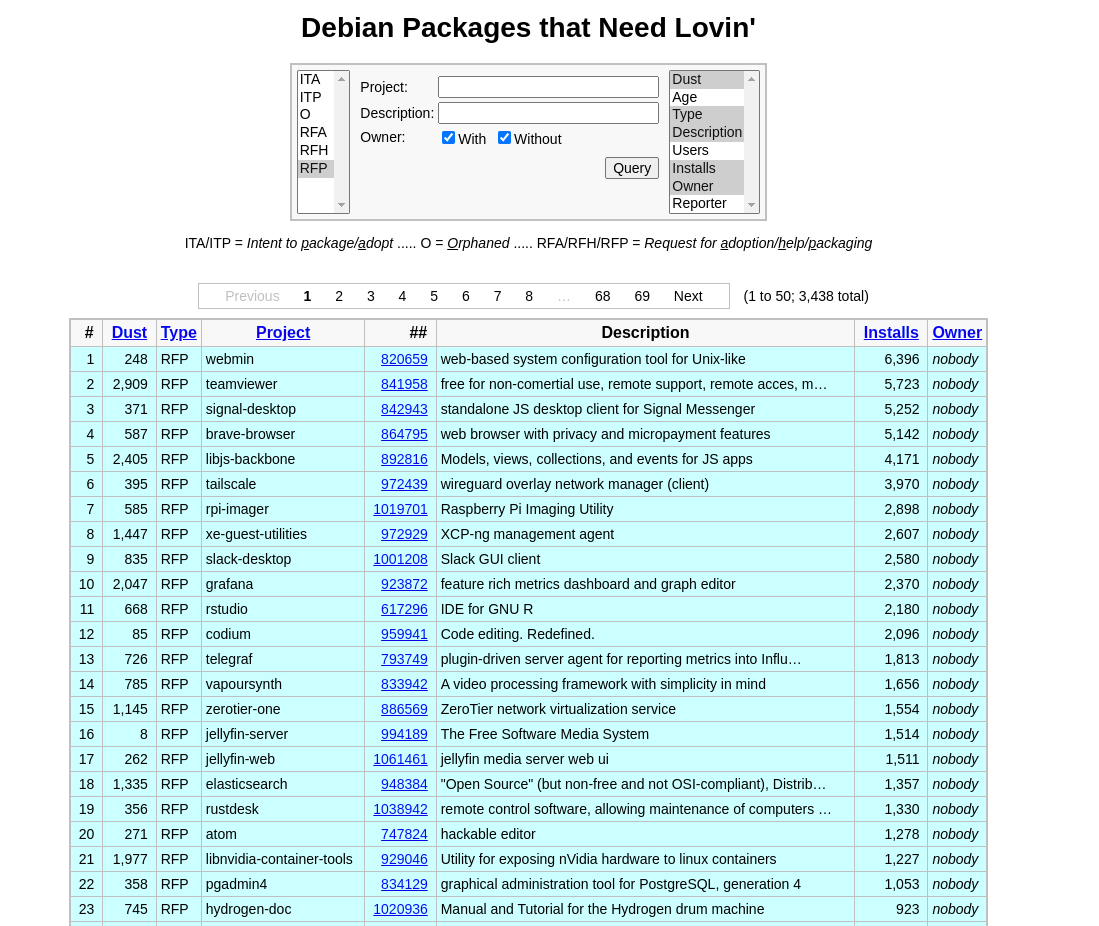
\includegraphics[width=0.7\linewidth]{images/rfp}
		\label{fig:rfp}
	\end{figure}
\end{frame}

\begin{frame}
 \frametitle{RFH}
    \begin{figure}
		\centering
		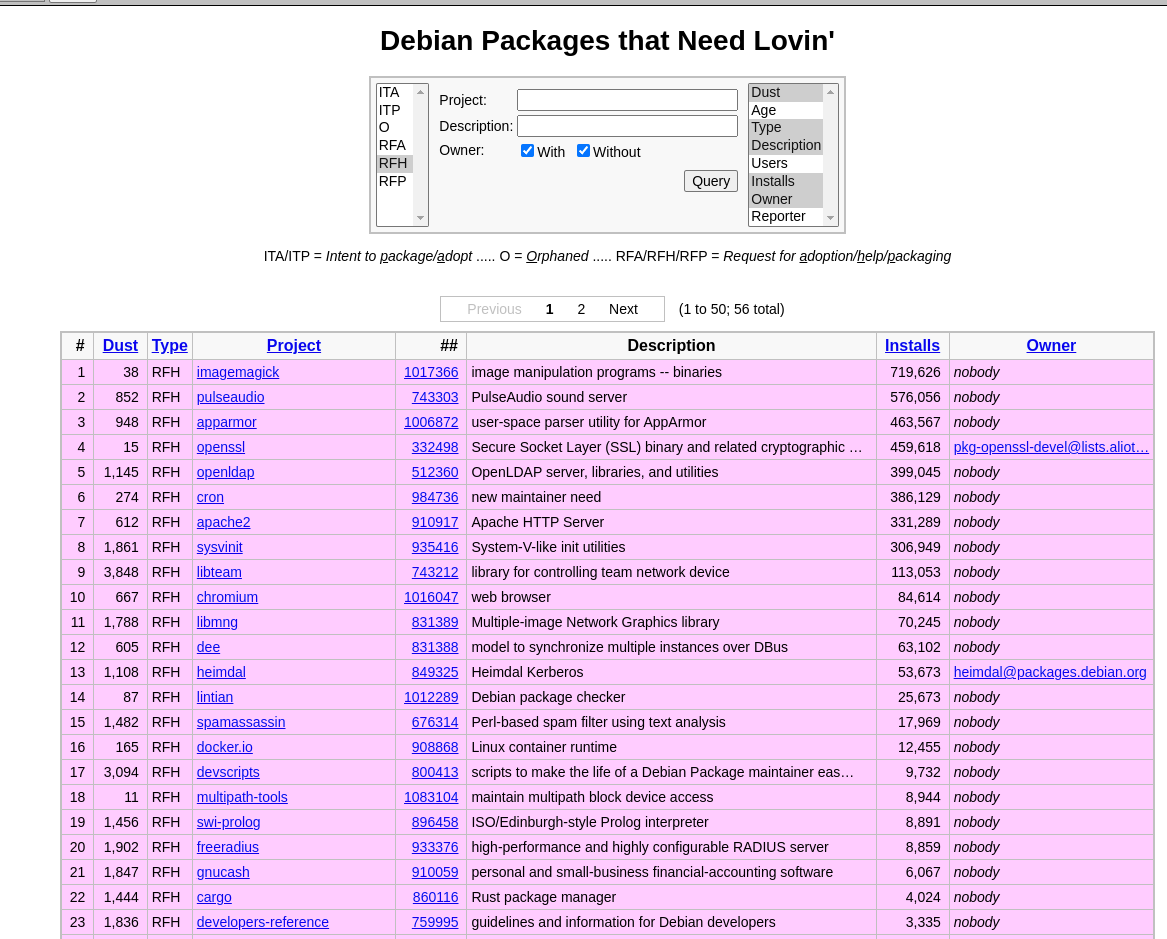
\includegraphics[width=0.7\linewidth]{images/rfh}
		\label{fig:rfh}
	\end{figure}
\end{frame}

\begin{frame}
 \frametitle{Adoptando un paquete}
    \begin{figure}
		\centering
		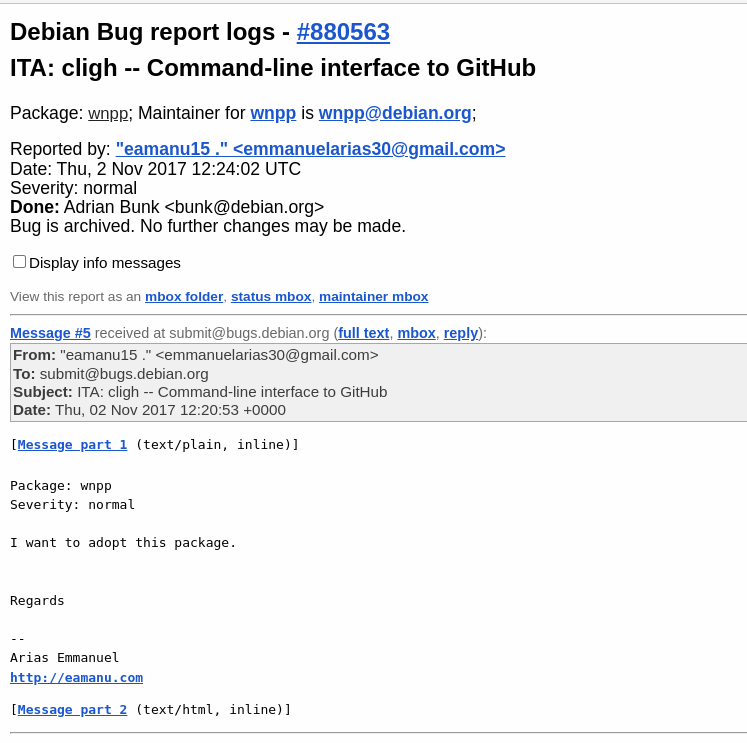
\includegraphics[width=0.7\linewidth]{images/ita}
		\label{fig:rfh}
	\end{figure}
\end{frame}

\begin{frame}
 \frametitle{2 meses después}
    \begin{figure}
		\centering
		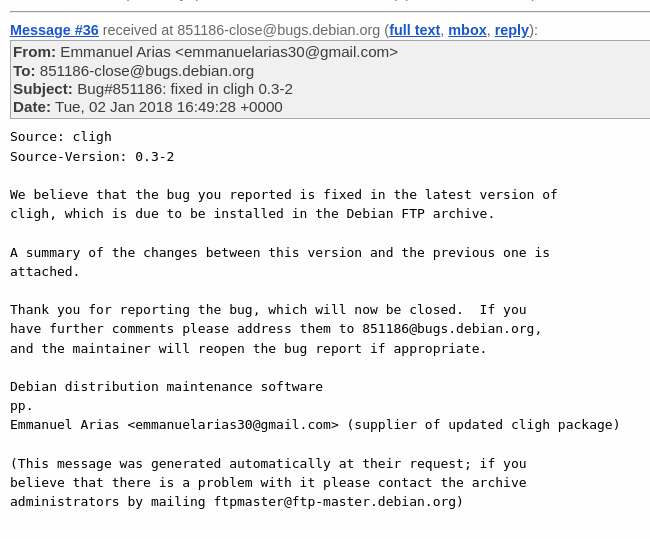
\includegraphics[width=0.7\linewidth]{images/ita2}
		\label{fig:rfh}
	\end{figure}
\end{frame}

\begin{frame}
 \frametitle{Mi primer bug reportado}
    \begin{figure}
		\centering
		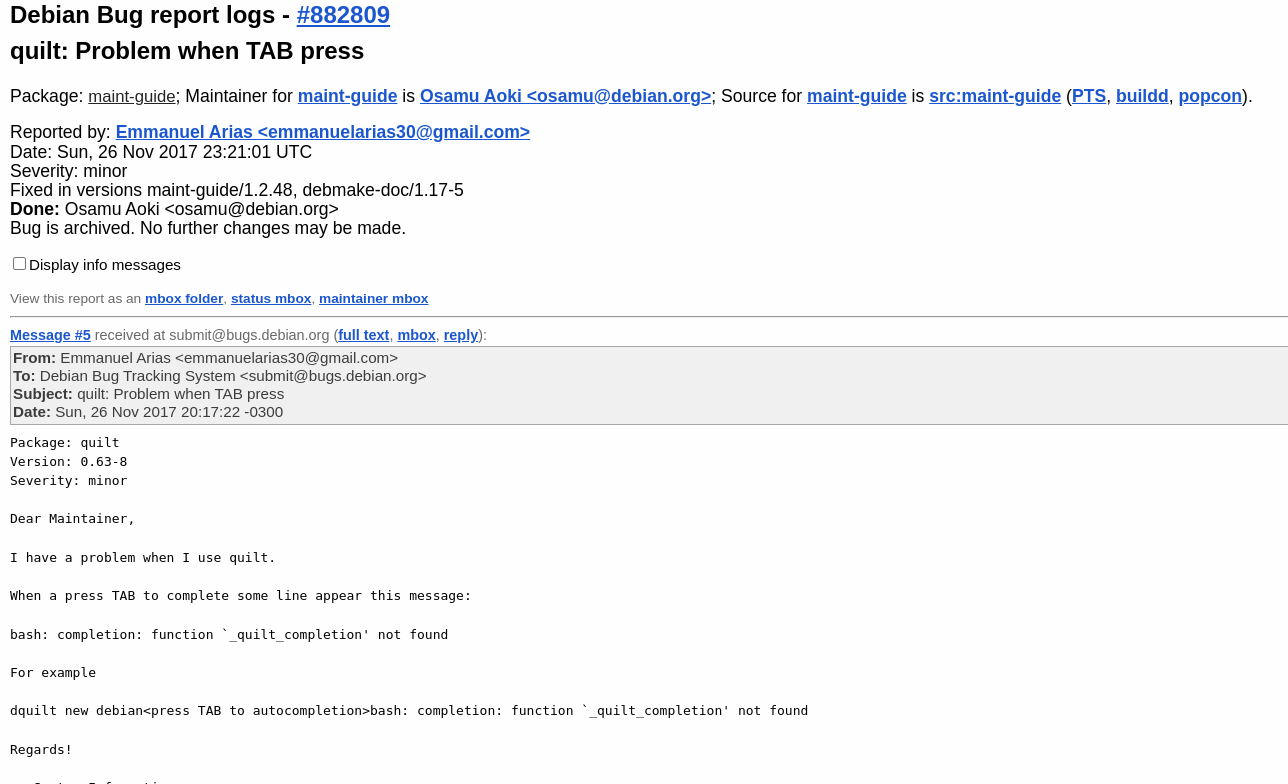
\includegraphics[width=0.7\linewidth]{images/bug}
		\label{fig:rfh}
	\end{figure}
\end{frame}

\begin{frame}
  \centering
  \Huge ¿Cuáles son los pasos dentro de Debian?
\end{frame}

\begin{frame}
  \frametitle {Pasos dentro de Debian}
  \begin{itemize}
    \item Debian Contributor \pause
    \item Debian Maintainer \pause
    \item Debian Developer
  \end{itemize}
\end{frame}

\begin{frame}
  \frametitle {Siguiente paso: Debian Maintainer}
      \begin{figure}
		\centering
		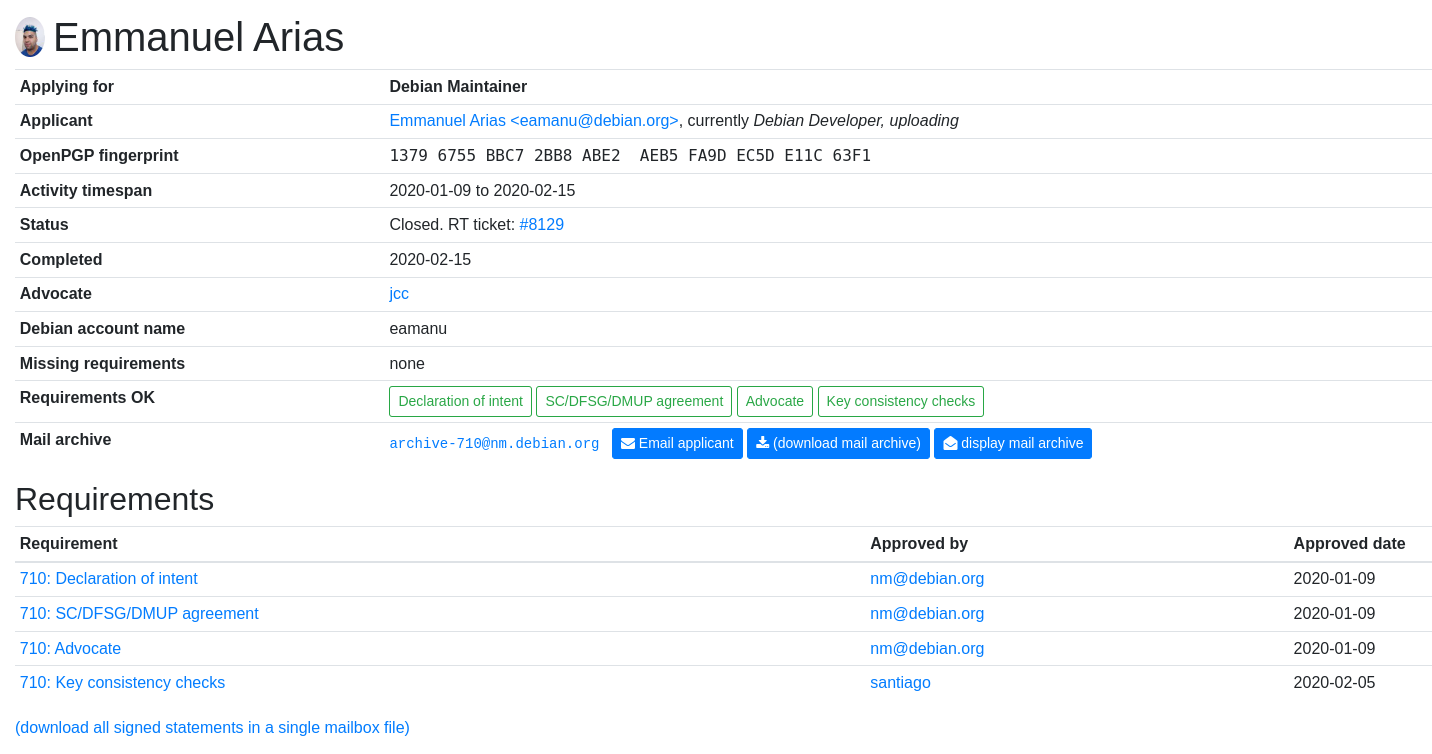
\includegraphics[width=0.7\linewidth]{images/DM}
		\label{fig:dm}
	\end{figure}
\end{frame}

\begin{frame}
  \frametitle {Siguiente paso: Debian Developer}
      \begin{figure}
		\centering
		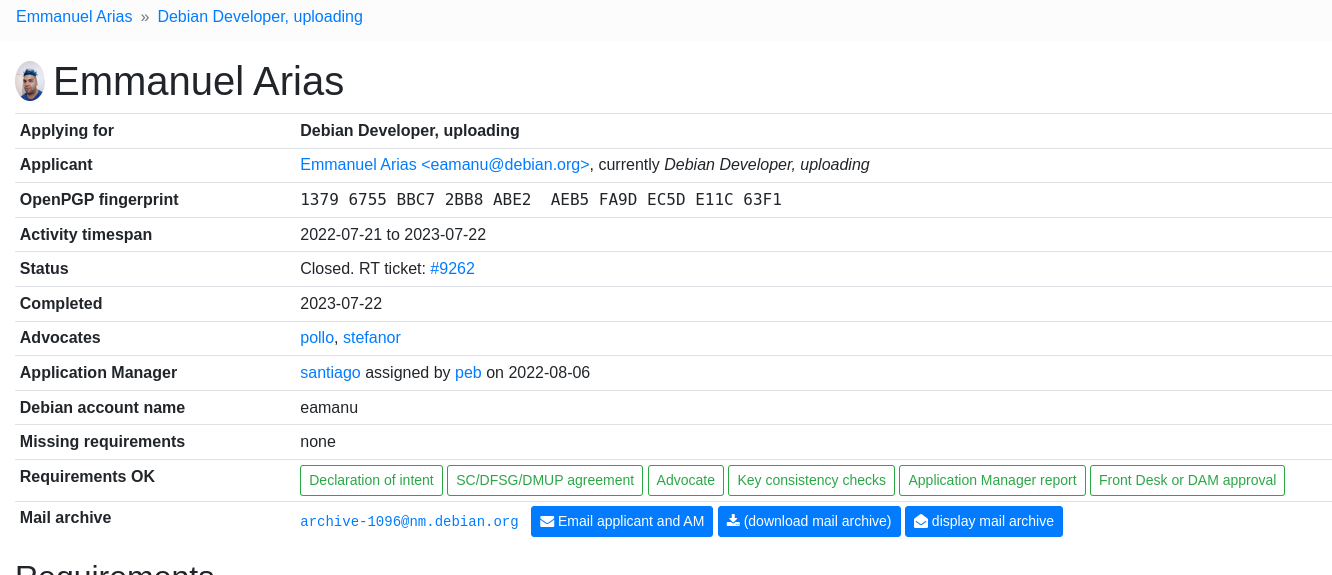
\includegraphics[width=0.7\linewidth]{images/dd}
		\label{fig:dd}
	\end{figure}
\end{frame}

\begin{frame}
  \centering
  \Huge Siguiente paso: Agrandar la comunidad Debian
\end{frame}

\begin{frame}
  \frametitle {Siguiente paso: Agrandar la comunidad Debian}
      \begin{figure}
		\centering
		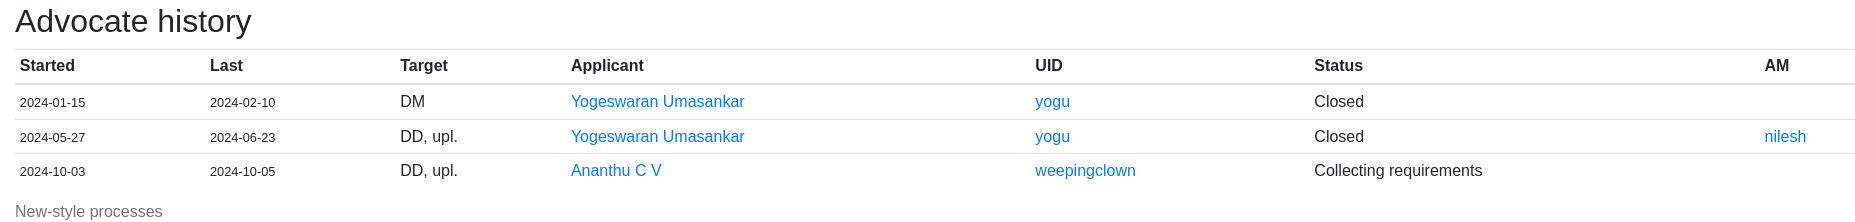
\includegraphics[width=0.7\linewidth]{images/advocate}
		\label{fig:dd}
	\end{figure}
\end{frame}

\begin{frame}
  \frametitle {¿Qué tareas puedo realizar?}
  \begin{itemize}
    \item Coding and Maintaining Packages \pause
    \item Testing and Bug Squashing \pause
    \item Writing Documentation and Tagging Packages \pause
    \item Translating and Localizing \pause
    \item Helping other Users \pause
    \item Organizing Events \pause
    \item Use Debian and talk about it
  \end{itemize}
\end{frame}

\begin{frame}
  \centering
  \huge Ultimo Consejo: paciencia, paciencia, paciencia.
\end{frame}

\begin{frame}
  \centering
  \Huge Gracias!!!
\end{frame}

\end{document}
